\documentclass[11pt,a4paper]{article}
\usepackage[T1]{fontenc}
\usepackage[utf8]{inputenc}
\usepackage{lmodern}
\usepackage[margin=26mm,headheight=14pt]{geometry}
\usepackage{amsmath,amssymb,amsthm,mathtools,bm}
\usepackage{microtype,booktabs,array,longtable,graphicx,enumitem,needspace}
\usepackage{xcolor,xurl}
\usepackage[colorlinks=true,linkcolor=blue!45!black,citecolor=blue!45!black,urlcolor=blue!45!black]{hyperref}
\usepackage{bookmark,fancyhdr}
\makeatletter
\renewcommand*{\l@subsection}{\@dottedtocline{2}{1.5em}{2.9em}}
\makeatother
\pagestyle{fancy}\fancyhf{}
\fancyhead[L]{\small The lower critical endpoint}\fancyhead[R]{\small Research article}
\fancyfoot[C]{\thepage}\renewcommand{\headrulewidth}{.3pt}
\setlength{\parskip}{3.5pt}\setlength{\parindent}{1.1em}
\setlength{\emergencystretch}{2em}
\numberwithin{equation}{section}
\newtheorem{theorem}{Theorem}[section]
\newtheorem{proposition}[theorem]{Proposition}
\newtheorem{lemma}[theorem]{Lemma}
\newtheorem{corollary}[theorem]{Corollary}
\theoremstyle{definition}
\newtheorem{definition}[theorem]{Definition}
\newtheorem{example}[theorem]{Example}
\theoremstyle{remark}
\newtheorem{remark}[theorem]{Remark}
\DeclareMathOperator{\Li}{Li}
\DeclareMathOperator{\Var}{Var}
\DeclareMathOperator{\Rea}{Re}
\DeclareMathOperator{\Eone}{E_1}
\newcommand{\R}{\mathbb R}\newcommand{\C}{\mathbb C}
\newcommand{\N}{\mathbb N}\newcommand{\E}{\mathbb E}\newcommand{\Prob}{\mathbb P}
\newcommand{\dd}{\,\mathrm d}\newcommand{\ii}{\mathrm i}
\newcommand{\ep}{\varepsilon}\newcommand{\la}{\lambda}
\newcommand{\rhob}{\rho_0}\newcommand{\ee}{\mathrm e}
\newcommand{\HH}{\mathcal H}\newcommand{\RR}{\mathcal R}
\newcommand{\coef}[1]{[#1]}
\newcommand{\repo}{\texttt{ProveIt}}
\hypersetup{pdftitle={Through the Lower Critical Endpoint: Exponentially Coalescing Folds, Landau Transseries, and Conditional Action Budgets},pdfauthor={Research draft prepared for Vladimir Reshetnikov},pdfsubject={Polylogarithmic exponential feedback, uniform lower-endpoint asymptotics, convergent inversion and conditioned Poisson extremes}}
\begin{document}
\hypersetup{pageanchor=false}
\begin{titlepage}
\vspace*{8mm}
\noindent{\small\scshape Transseries \quad / \quad asymptotic inversion \quad / \quad conditioned jumps}
\vspace{17mm}
\begin{center}
{\LARGE\bfseries Through the Lower Critical Endpoint\par}
\vspace{7mm}
{\Large Exponentially Coalescing Folds,\par Landau Transseries,\par and Conditional Action Budgets\par}
\vspace{12mm}
{Research draft prepared for Vladimir Reshetnikov\par}
\vspace{3mm}{29 September 2026\par}
\end{center}
\vspace{10mm}
\begin{abstract}
We study the lower-endpoint problem for the countable-action equation
\(U=c\Li_{2+\ep}(q\ee^U)\), where \(\alpha=1+\ep\downarrow1\).
On the interior-fold side, an exact saddle normalization removes the
apparent pole at \(\ep=0\). It yields a uniform coefficient theorem with no
restriction on \(\ep\log(1/\delta)\), where \(\ee^{-\delta}\) is the fold
location. At the endpoint, \(\delta\sim\ee^{-1/c}\), and the crossover
variable is \(\la=nc\delta\). The limiting coefficient profile is an
explicit transform of the classical Landau density. We prove its
all-orders finite-coefficient correction scheme, a convergent Lambert
inverse chart and a uniform two-sheet fold chart. We also identify the
first obstruction to extending the compact-crossover formula into the
Gaussian range: a relative factor \(\exp(\la\delta/4)\).

For a truncation to actions \(j\le M\), we obtain the exact limiting
conditional profile and prove that coefficient preservation is equivalent
to \(M\delta\to\infty\) in a compact crossover window. Its loss has a sharp
doubly exponential equivalent, including the prefactor. Consequently the
scaled action budget for a small limiting loss \(h\) grows like
\(\la\log\log(1/h)\), not like \(\log(1/h)\). Proofs, exact algebraic checks,
numerical diagnostics, a source audit, and further research questions are
included.
\end{abstract}
\vfill
\noindent\textbf{Scope.} This is a conventional mathematical research draft.
It resolves a specified interior-fold part of a repository-local lower-endpoint
question, not every critical-coupling path at \(\alpha=1\). The classical
Landau law, Lagrange inversion, and Poisson insertion identities are not
claimed as new. Global priority, independent refereeing, and Lean verification
are not asserted.
\end{titlepage}
\hypersetup{pageanchor=true}\setcounter{page}{1}
\begingroup
\small
\setlength{\parskip}{0pt}
\tableofcontents
\endgroup
\clearpage

\section{The question and the contribution}
\label{sec:intro}

\subsection{The repository boundary being addressed}
The \repo\ package \emph{Beyond Finite-Action Folds} studies positive
countable-action equations with tail \(j^{-1-\alpha}\) for
\(1<\alpha<2\). Its later editorial cross-references record work at the
upper endpoint and explicitly leave the lower endpoint \(\alpha\to1\)
unresolved \cite{repo-critical}. The present paper addresses the pure-tail
family
\begin{equation}\label{eq:model}
 U_{\ep,c}(q)=c\sum_{j\ge1}\frac{q^j\ee^{jU_{\ep,c}(q)}}{j^{2+\ep}}
             =c\Li_{2+\ep}(q\ee^{U_{\ep,c}(q)}),
 \qquad c>0,\quad \ep\ge0.
\end{equation}
Its tail exponent is \(\alpha=1+\ep\). The ordinary coefficients are
\(u_n(\ep,c)=\coef{q^n}U_{\ep,c}(q)\); they are not multiplied by \(n!\).

For \(\ep>0\), the boundary-critical coupling is
\(c_{\mathrm b}=1/\zeta(1+\ep)\). For \(c>c_{\mathrm b}\), the physical
branch encounters an interior fold before the polylogarithmic boundary.
At \(\ep=0\), every \(c>0\) has such a fold. As \(c\downarrow0\), its
location approaches the boundary at an exponentially small distance.
This singular approach is not captured by putting \(\ep=0\) separately
in terms containing \(\Gamma(-1-\ep)\) and \(\zeta(1+\ep)\).

We normalize by the \emph{exact} fold location before taking a limit. This
produces one formula for all relative rates at which \(\ep\) and the fold
distance vanish. It also exposes a conditional large-jump phenomenon:
a very large positive jump must be compensated by an exceptionally
unlikely negative fluctuation of the remaining centered cloud.
That compensation changes the action-cutoff loss from an ordinary
exponential tail into a doubly exponential one.

\subsection{What is inherited and what is established here}
The substitution \(t=q\ee^U\), its Lagrange coefficient identity, and the
conditional-Poisson representation already occur in the repository's
critical-Hahn article \cite{repo-critical}. More generally, the connection
with simply generated trees and conditioned allocations is classical;
Janson gives an extensive treatment \cite{janson}. The polylogarithm
continuation formula is classical \cite[Eq.~25.12.12]{dlmf-polylog}.
The Landau distribution is likewise an established stable law, not a new
special function introduced by this paper \cite{bulyak}.

The results proved below are the following linked, model-specific
statements. The distinction between a proved statement in this draft and
an established claim of publication priority is maintained throughout.
\begin{center}
\small
\begin{tabular}{p{.24\textwidth}p{.64\textwidth}}
\toprule
Result & Added content and boundary \\
\midrule
Exact confluence & A convergent normal form uniform through \(\ep=0\),
with no bound on \(\ep\log(1/\delta)\). \\
Coefficient crossover & A uniform additive error
\(O(\delta^{1-\eta})\) for \(0\le\ep\le\eta<1/2\) and compact positive
\(\la\)-windows; an all-orders expansion at \(\ep=0\). \\
Inverse charts & A genuinely convergent exponential-scale inverse and a
uniform two-sheet chart through the moving fold. \\
Matching obstruction & The factor \(\ee^{\ell/4}\) when
\(\la\to\infty\) and \(\la\delta\to\ell\); the compact-window theorem is
not silently used outside its range. \\
Conditional budget & A limiting cutoff profile, an if-and-only-if
preservation criterion, and a sharp doubly exponential tail with its
prefactor. \\
\bottomrule
\end{tabular}
\end{center}

\subsection{Limits that are deliberately not identified}
Three different limiting statements will appear. A \emph{coefficient
crossover} lets \(n\to\infty\), \(\delta\to0\), and possibly \(\ep\to0\),
with \(\la=nA\delta\) in a compact subset of \((0,\infty)\).
A \emph{profile asymptotic} subsequently lets \(\la\) tend to zero or
infinity, or the scaled cutoff \(m\) tend to infinity. A \emph{Gaussian
matching theorem} has its own proof for \(\la\to\infty\).
Only the last of these justifies a simultaneous unbounded-\(\la\) limit.
Similarly, the small-tolerance action budget at the end of the paper is a
statement about the limiting profile, not an unproved finite-\(n\)
certificate at an arbitrarily small tolerance.

\section{Exact coordinates and coefficients}
\label{sec:exact}
Fix \(0\le\ep\le\eta<1/2\). For \(\delta>0\), define
\begin{align}
 \tau&=\ee^{-\delta},&
 c&=\frac1{\Li_{1+\ep}(\ee^{-\delta})},\label{eq:c}\\
 A&=c\Gamma(1-\ep)\delta^\ep,&
 \la&=nA\delta.\label{eq:A}
\end{align}
All these parameters are positive. The choice \eqref{eq:c} parametrizes
the entire interior-fold side for \(\ep>0\), and all positive couplings
for \(\ep=0\). Introduce
\begin{align}
 Q(x)&=-x-c\Li_{2+\ep}(\ee^{-x}),\label{eq:Q}\\
 \rhob&=\exp\{-c\zeta(2+\ep)\},&
 \rho&=\exp\{Q(\delta)\}.\label{eq:rhos}
\end{align}
The notation \(Q(0)\) denotes the continuous boundary value \(\log\rhob\).
Unless otherwise stated, complex logarithms are principal.

\begin{proposition}[Exact real fold]\label{prop:fold}
Under \eqref{eq:c}, \(Q'(\delta)=0\) and
\[
 Q''(\delta)=-c\Li_\ep(\ee^{-\delta})<0.
\]
The physical real branch is parametrized by
\[
 t=q\ee^U,\qquad U=c\Li_{2+\ep}(t),\qquad
 q=t\exp\{-c\Li_{2+\ep}(t)\},\qquad 0\le t\le\tau.
\]
At \(\ep=0\), one has the exact identities
\begin{equation}\label{eq:essential}
 \tau=1-\ee^{-1/c},\qquad
 \delta=-\log(1-\ee^{-1/c}),\qquad A=c.
\end{equation}
Consequently \(\delta\sim\ee^{-1/c}\) as \(c\downarrow0\).
\end{proposition}
\begin{proof}
Differentiating the polylogarithm series inside its disk of convergence
and then substituting \(t=\ee^{-x}\) gives
\(Q'(x)=-1+c\Li_{1+\ep}(\ee^{-x})\) and
\(Q''(x)=-c\Li_\ep(\ee^{-x})\). The latter is negative on the positive
real axis. Equation \eqref{eq:c} therefore gives the unique stationary
point. Equivalently, \(t\mapsto t\ee^{-c\Li_{2+\ep}(t)}\) is strictly
increasing up to \(t=\tau\). The formal solution at zero is unique by
coefficient induction and is analytic there by the implicit function
theorem. The displayed parametrization continues its positive real
branch to the fold. Finally,
\(\Li_1(t)=-\log(1-t)\) turns the fold equation into
\(-c\log(1-\tau)=1\), proving \eqref{eq:essential}.
\end{proof}

\begin{proposition}[Classical coefficient and conditioning identities]
\label{prop:poisson}
For every integer \(n\ge1\),
\begin{equation}\label{eq:lagrange}
 u_n(\ep,c)=\frac1n\coef{t^n}\exp\{nc\Li_{2+\ep}(t)\}.
\end{equation}
Let \(N_j\) be independent Poisson variables with means
\begin{equation}\label{eq:intensities}
 \mu_j=nc\frac{\ee^{-\delta j}}{j^{2+\ep}},\qquad
 S=\sum_{j\ge1}jN_j.
\end{equation}
Then \(\E S=n\), and
\begin{equation}\label{eq:exact-mass}
 u_n=\frac{\rho^{-n}}n\Prob(S=n).
\end{equation}
If \(u_{n,M}\) is the coefficient for the equation with actions
\(1\le j\le M\), then
\begin{equation}\label{eq:exact-ratio}
 \frac{u_{n,M}}{u_n}
 =\Prob(N_j=0\text{ for every }j>M\mid S=n).
\end{equation}
In particular this ratio is in \([0,1]\), increases with \(M\), and is
exactly one for \(M\ge n\).
\end{proposition}
\begin{proof}
Put \(t=q\exp(c\Li_{2+\ep}(t))\). Lagrange inversion gives
\[
 \coef{q^n}c\Li_{2+\ep}(t(q))
 =\frac1n\coef{t^{n-1}}c\Li'_{2+\ep}(t)
                         \ee^{nc\Li_{2+\ep}(t)}
 =\frac1n\coef{t^n}\ee^{nc\Li_{2+\ep}(t)}.
\]
The last equality follows by differentiating the exponential and
comparing its coefficient of degree \(n-1\).
The generating function of \(S\) is
\[
 \E z^S=\exp\{nc(\Li_{2+\ep}(\tau z)-\Li_{2+\ep}(\tau))\}.
\]
Its coefficient of \(z^n\), together with \(\tau=\ee^{-\delta}\), yields
\eqref{eq:exact-mass}. The mean is
\(nc\Li_{1+\ep}(\tau)=n\). The total Poisson intensity is finite, so the
random sum is well defined. Requiring no jump above \(M\) replaces the
positive-degree part of the generating exponent by its truncation while
retaining the \emph{full} zero-event factor. Dividing the resulting
coefficient by the unrestricted one proves \eqref{eq:exact-ratio}.
These identities are included for clarity, not claimed as new results.
\end{proof}

\section{A convergent normal form through the lower endpoint}
\label{sec:normal}
Define, for \(\Rea s>0\),
\begin{equation}\label{eq:f}
 f_\ep(s)=
 \begin{cases}
 \displaystyle\frac{s-s^{1+\ep}/(1+\ep)}\ep,&\ep\ne0,\\[5pt]
 s(1-\log s),&\ep=0.
 \end{cases}
\end{equation}
The singularity at \(\ep=0\) is removable. Direct differentiation gives
\begin{equation}\label{eq:f-derivatives}
 f_\ep'(s)=\frac{1-s^\ep}{\ep},\qquad
 f_\ep'(1)=0,\qquad f_\ep''(1)=-1,\qquad
 f_\ep(1)=\frac1{1+\ep},
\end{equation}
with the continuous interpretation of the first expression.

\begin{theorem}[Exact confluent normal form]\label{thm:normal}
For \(0\le\ep\le\eta<1/2\), \(0<\delta<2\pi\), and
\(\Rea s>0\), \(|\delta s|<2\pi\),
\begin{equation}\label{eq:normal}
 F_{\ep,\delta}(s):=\frac{Q(\delta s)-Q(0)}{A\delta}
       =f_\ep(s)+R_{\ep,\delta}(s),
\end{equation}
where the following series is convergent:
\begin{equation}\label{eq:R}
 R_{\ep,\delta}(s)=
 \frac1{\Gamma(1-\ep)}
 \sum_{k\ge2}\frac{(-1)^k\zeta(2+\ep-k)}{k!}
   \delta^{k-1-\ep}(ks-s^k).
\end{equation}
For every compact \(K\subset\{\Rea s>0\}\),
\begin{equation}\label{eq:normal-bound}
 \sup_{s\in K}|R_{\ep,\delta}(s)|
 \le C_{K,\eta}\delta^{1-\ep}
 \le C_{K,\eta}\delta^{1-\eta}\qquad(0<\delta\le\delta_K).
\end{equation}
The same bound holds for each fixed number of derivatives in \(s\).
In particular no assumption on \(\ep\log(1/\delta)\) is made.
\end{theorem}
\begin{proof}
For nonintegral order, the classical convergent continuation formula is
\begin{equation}\label{eq:jonquiere}
 \Li_{2+\ep}(\ee^{-x})
 =\Gamma(-1-\ep)x^{1+\ep}
  +\sum_{k\ge0}\zeta(2+\ep-k)\frac{(-x)^k}{k!},
 \qquad |x|<2\pi,\quad |\arg x|<\pi.
\end{equation}
This is \cite[Eq.~25.12.12]{dlmf-polylog}; the separate singular terms
at integral order must first be combined. The fold equation, using its
derivative version, says
\[
 c\zeta(1+\ep)-1
 =-c\Gamma(-\ep)\delta^\ep
  -c\sum_{j\ge1}\zeta(1+\ep-j)\frac{(-\delta)^j}{j!}.
\]
Insert this equality into the linear term of
\(Q(\delta s)-Q(0)\). The gamma identities
\[
 -\Gamma(-\ep)=\frac{\Gamma(1-\ep)}\ep,
 \qquad
 \Gamma(-1-\ep)=\frac{\Gamma(1-\ep)}{\ep(1+\ep)}
\]
produce \(f_\ep\). Reindexing the remaining linear sum with \(k=j+1\)
produces exactly \(ks-s^k\), with the sign shown in \eqref{eq:R}.

After this combination, every coefficient in \eqref{eq:R} is regular
for \(0\le\ep\le\eta\); the zeta arguments there stay away from its
pole. The power series is normally convergent when \(\delta\) and
\(\delta s\) stay in smaller disks. Passing to \(\ep=0\) is therefore
legitimate. For completeness, uniform geometric coefficient bounds can
be obtained from the zeta functional equation and Stirling's formula:
for any \(r<2\pi\), the quantities
\(|\zeta(2+\ep-k)|/k!\) are bounded by \(C_{r,\eta}r^{-k}\)
uniformly in \(\ep\). Alternatively they follow by Cauchy estimates
for the regular analytic remainder of \eqref{eq:jonquiere} on a smaller
disk. Factoring out \(\delta^{1-\ep}\) now proves
\eqref{eq:normal-bound}; differentiated series give the derivative bounds.
\end{proof}

\begin{corollary}[Endpoint coefficients and fold value]\label{cor:normal-zero}
At \(\ep=0\), \(R_{0,\delta}\) is analytic in \(\delta\), and
\begin{align}
 R_{0,\delta}(s)
 &=\delta\left(-\frac{s}{2}+\frac{s^2}{4}\right)
   +\frac{\delta^2}{72}(3s-s^3)
   -\frac{\delta^4}{14400}(5s-s^5)+O_K(\delta^6),\label{eq:Rzero}\\
 F_{0,\delta}(1)
 &=1-\frac\delta4+\frac{\delta^2}{36}
                      -\frac{\delta^4}{3600}+O(\delta^6),\label{eq:fold-value}\\
 F_{0,\delta}''(1)&=-\frac{\delta}{\ee^\delta-1}.
 \label{eq:fold-curvature}
\end{align}
Here \(F'_{0,\delta}(1)=0\) holds exactly, not just asymptotically.
\end{corollary}
\begin{proof}
Use \(\zeta(0)=-1/2\), \(\zeta(-1)=-1/12\),
\(\zeta(-2r)=0\) for positive integers \(r\), and
\(\zeta(-3)=1/120\) in \eqref{eq:R}. Every summand has derivative zero
at \(s=1\). Finally,
\(F''_{0,\delta}(1)=\delta Q''(\delta)/c
=-\delta\Li_0(\ee^{-\delta})\), proving \eqref{eq:fold-curvature}.
\end{proof}

\begin{proposition}[All rates of confluence]\label{prop:rates}
As \(\ep\downarrow0\) and \(\delta\downarrow0\), jointly,
\begin{equation}\label{eq:coupling-uniform}
 \frac1c=\frac{1-\delta^\ep}\ep+O(1),
 \qquad
 c\sim\frac\ep{1-\delta^\ep},
\end{equation}
with the quotients interpreted continuously at \(\ep=0\).
If \(L=\log(1/\delta)\) and \(r=\ep L\), then
\(c\sim1/L\) for \(r\to0\),
\(c\sim\ep/(1-\ee^{-r_0})\) for \(r\to r_0\in(0,\infty)\),
and \(c\sim\ep\) for \(r\to\infty\).
\end{proposition}
\begin{proof}
The derivative form of \eqref{eq:jonquiere} gives
\[
 \Li_{1+\ep}(\ee^{-\delta})
 =\zeta(1+\ep)-\frac{\Gamma(1-\ep)}\ep\delta^\ep+O(\delta).
\]
The functions \(\zeta(1+\ep)-1/\ep\) and
\((\Gamma(1-\ep)-1)/\ep\) are bounded near zero. This proves the first
formula, uniformly since \(0\le\delta^\ep\le1\). Its leading term is
\(L(1-\ee^{-r})/r\), which tends to infinity for every joint approach:
when \(r\le1\) it is comparable to \(L\), and when \(r\ge1\) it is
comparable to \(1/\ep\). The additive \(O(1)\) is therefore relatively
negligible. The stated regimes follow.
\end{proof}

\section{Uniform coefficient crossover and its Landau limit}
\label{sec:crossover}

\subsection{The limiting density and a domination lemma}
For \(\la>0\), define
\begin{equation}\label{eq:H}
 \HH_\ep(\la)=\frac1{2\pi\ii}
   \int_{1-\ii\infty}^{1+\ii\infty}\exp\{-\la f_\ep(s)\}\dd s.
\end{equation}
The integral is absolutely convergent. We write \(\HH=\HH_0\).
A useful probabilistic normalization is the L\'evy measure
\begin{equation}\label{eq:nu-eps}
 \nu_{\ep,\la}(\dd x)=
 \frac\la{\Gamma(1-\ep)}\ee^{-x}x^{-2-\ep}\dd x,
 \qquad x>0.
\end{equation}
Although its first moment at zero is infinite, its second moment is
finite. Hence compensated integration of the jumps, defined as an
\(L^2\) limit, gives a centered random variable \(Y_{\ep,\la}\) with
characteristic exponent
\begin{align}
 \Psi_{\ep,\la}(u)
 &=\int_0^\infty(\ee^{\ii ux}-1-\ii ux)\nu_{\ep,\la}(\dd x)\label{eq:psi-int}\\
 &=\la\{f_\ep(1)-f_\ep(1-\ii u)\}.\label{eq:psi}
\end{align}
At zero,
\begin{equation}\label{eq:psi-zero}
 \Psi_{0,\la}(u)=\la\{(1-\ii u)\log(1-\ii u)+\ii u\}.
\end{equation}
Its density will be denoted by \(g_{\ep,\la}\).

\begin{lemma}[Decay, analyticity, and positivity]\label{lem:density}
For \(0\le\ep\le\eta<1/2\) and \(\la\) in a compact positive interval,
\[
 |\exp\Psi_{\ep,\la}(u)|\le C\exp(-b|u|^{1+\ep})
 \quad (|u|\ge1),
\]
where \(C,b>0\) are uniform. The densities \(g_{\ep,\la}\) exist, are
real analytic, and are strictly positive on \(\R\). Moreover
\begin{equation}\label{eq:g0-H}
 g_{\ep,\la}(0)=\ee^{\la/(1+\ep)}\HH_\ep(\la)>0.
\end{equation}
For each fixed \(m>0\), the same analyticity and positivity statements
hold when \(\nu_{\ep,\la}\) is restricted to \((0,m]\).
\end{lemma}
\begin{proof}
For \(|u|\ge1\), integrate the nonnegative quantity
\((1-\cos ux)\ee^{-x}x^{-2-\ep}\) over
\(x\in[a/|u|,b_0/|u|]\), where fixed
\(0<a<b_0<2\pi\) avoid zeros of \(1-\cos v\).
The resulting lower bound is a uniform positive multiple of
\(|u|^{1+\ep}\). For a restricted measure the same interval works as
soon as \(|u|\ge b_0/m\). Fourier inversion therefore gives a continuous
density, whose Fourier integral extends holomorphically to a strip.
It is a nonnegative real-analytic function and is not identically zero;
its real zeros are consequently isolated. Splitting the intensity into
two equal independent parts expresses this density as the convolution
of two such densities. Each factor is positive almost everywhere, so
the convolution is positive at every real argument. This proves strict
positivity, including in the restricted case. Formula \eqref{eq:g0-H}
follows from \eqref{eq:psi}. Equation \eqref{eq:psi} itself may be checked
by differentiating twice in \(u\), evaluating the elementary gamma
integral, and matching value and first derivative at zero.
\end{proof}

\begin{lemma}[Uniform lattice attenuation]\label{lem:lattice}
Let \(\mu_j\) be given by \eqref{eq:intensities} and set
\[
 D(\theta)=\sum_{j\ge1}\mu_j(1-\cos j\theta).
\]
There exist fixed \(\theta_0,b>0\), uniform for small \(\delta\),
\(0\le\ep\le\eta\), and compact positive \(\la\)-windows, such that
\begin{align}
 D(\theta)&\ge b\la(\theta/\delta)^2,
       &&|\theta|\le\delta,\label{eq:atten-small}\\
 D(\theta)&\ge b\la|\theta/\delta|^{1+\ep},
       &&\delta\le|\theta|\le\theta_0,\label{eq:atten-mid}\\
 D(\theta)&\ge bnc,
       &&\theta_0\le|\theta|\le\pi.\label{eq:atten-far}
\end{align}
\end{lemma}
\begin{proof}
For \(|\theta|\le\delta\), take integers
\(j\in[1/(2\delta),1/\delta]\). There are order \(1/\delta\) of them,
\(\ee^{-\delta j}\) is bounded below, and
\(1-\cos j\theta\ge b_1j^2\theta^2\). Their sum is at least
\(b_2nc\delta^{\ep-1}\theta^2\), which equals a positive uniform
multiple of \(\la(\theta/\delta)^2\).
For \(\delta\le|\theta|\le\theta_0\), use
\(j\in[a/|\theta|,b_0/|\theta|]\) with fixed suitable \(a,b_0\).
Choosing \(\theta_0\) small ensures enough integers in this interval;
the phase is away from a multiple of \(2\pi\), and
\(\ee^{-\delta j}\) stays bounded below. The sum is at least
\(b_3nc|\theta|^{1+\ep}\). Since
\(nc\delta^{1+\ep}=\la/\Gamma(1-\ep)\), this proves the middle bound.
For the last bound, the single \(j=1\) term suffices because
\(1-\cos\theta\) has a positive minimum on
\(\theta_0\le|\theta|\le\pi\).
\end{proof}

\subsection{A uniform theorem, not merely a formal substitution}
\begin{theorem}[Lower-endpoint coefficient crossover]\label{thm:crossover}
Fix \(\eta<1/2\) and \(0<\la_-<\la_+<\infty\). Uniformly over
\(0\le\ep\le\eta\), \(\delta\downarrow0\), and integers \(n\ge1\) for
which \(\la=nA\delta\in[\la_-,\la_+]\),
\begin{equation}\label{eq:crossover}
 u_n(\ep,c)=\rhob^{-n}\frac\delta n
 \left\{\HH_\ep(\la)+O(\delta^{1-\eta})\right\}.
\end{equation}
The error is additive inside braces, and is also a relative
\(O(\delta^{1-\eta})\) error because the profile is bounded away from
zero on these compact parameter sets. If additionally \(\ep\to0\), then
\(\HH_\ep(\la)\to\HH(\la)\) uniformly on compact positive
\(\la\)-intervals. In particular no bound on
\(\ep\log(1/\delta)\) is required for the joint limit.
\end{theorem}
\begin{proof}
Cauchy's coefficient integral on \(|t|=\ee^{-\delta}\), with
\(t=\ee^{-\delta+\ii\theta}\), is exactly
\begin{equation}\label{eq:integral-exact}
 \frac{n\rhob^n u_n}{\delta}
 =\frac1{2\pi}\int_{-\pi/\delta}^{\pi/\delta}
  \exp\{-\la F_{\ep,\delta}(1-\ii u)\}\dd u.
\end{equation}
There is no extra factor \(\ee^{-\delta s}\) in this formula: we are
extracting a coefficient of \(U\), and the original contour element is
\(\dd t/t\). Including such a factor would give incorrect correction
coefficients.

The value of the integrand's modulus at \(u=0\) is uniformly bounded.
Its remaining modulus is multiplied by
\(\exp\{-D(\delta u)\}\). Lemma~\ref{lem:lattice} therefore supplies an
integrable dominating function on the central and intermediate arcs;
the far arc has integral at most
\(C\delta^{-1}\exp(-bnc)\), smaller than every fixed positive power of
\(\delta\). The normal form gives pointwise convergence of the central
integrand to \(\exp\{-\la f_\ep(1-\ii u)\}\).

To obtain the stated rate rather than only convergence, fix a small
\(r>0\). The convergent series \eqref{eq:R} gives, on
\(|\delta(1-\ii u)|\le r\),
\begin{equation}\label{eq:R-growing}
 |R_{\ep,\delta}(1-\ii u)|
 \le C\delta^{1-\ep}(1+u^2).
\end{equation}
Both the exact exponent and the limiting exponent have real-part
attenuation at least \(b|u|^{1+\ep}-C\) for \(|u|\ge1\).
Using the integral formula for the difference of two exponentials, their
interpolated real parts have the same bound. The difference of the
integrands is thus bounded by
\[
 C\delta^{1-\ep}(1+u^2)\exp(-b|u|^{1+\ep}).
\]
Its integral is \(O(\delta^{1-\eta})\). Beyond this growing arc the
attenuation estimates make both tails exponentially small in a
positive power of \(1/\delta\). This proves \eqref{eq:crossover}.

Finally, \(f_\ep(s)\) is continuous at zero in \(\ep\), and the same
uniform domination applies to \eqref{eq:H}. Dominated convergence gives
continuity of the profile in \((\ep,\la)\). Strict positivity from
Lemma~\ref{lem:density}, followed by compactness, gives the positive
lower bound and the claimed relative interpretation.
\end{proof}

\begin{corollary}[The essential crossover scale]\label{cor:scale}
At \(\ep=0\), the bounded positive crossover occurs at
\begin{equation}\label{eq:scale}
 \la=nc\delta\sim nc\ee^{-1/c},
 \qquad n\asymp\frac{\ee^{1/c}}c.
\end{equation}
Thus an exponentially close fold becomes visible only at an exponentially
large coefficient index. This is an index scale, not an additional
singularity of the original equation.
\end{corollary}
\begin{proof}
Combine \eqref{eq:essential} with \(A=c\) and the definition of \(\la\).
\end{proof}

\section{The Landau profile and an all-orders correction calculus}
\label{sec:landau}

\subsection{Identification with a classical density}
Define the Landau density in the following normalization:
\begin{equation}\label{eq:landau}
 p(x)=\frac1{2\pi\ii}\int_{a-\ii\infty}^{a+\ii\infty}
                \exp\{z\log z+xz\}\dd z,\qquad a>0.
\end{equation}
The value is independent of \(a\), by contour displacement and the
exponential decay on vertical lines. Different location and scale
conventions for this classical law are common \cite{bulyak}; equation
\eqref{eq:landau}, rather than a name alone, fixes our convention.

\begin{proposition}[Exact Landau identification]\label{prop:landau}
For every \(\la>0\),
\begin{align}
 \HH(\la)&=\frac1\la p(-1-\log\la),\label{eq:Hlandau}\\
 g_{0,\la}(y)&=\frac{\ee^{\la-y}}\la
      p\left(\frac y\la-1-\log\la\right).
 \label{eq:glandau}
\end{align}
The function \(p\) is strictly positive and integrates to one.
It also has the real Hankel representation
\begin{equation}\label{eq:hankel}
 p(x)=\frac1\pi\int_0^\infty
             \ee^{-t\log t-xt}\sin(\pi t)\dd t.
\end{equation}
\end{proposition}
\begin{proof}
In \eqref{eq:H} at \(\ep=0\), substitute \(z=\la s\).
The exponent becomes
\(z\log z+(-1-\log\la)z\), proving \eqref{eq:Hlandau}.
Fourier inversion of \eqref{eq:psi-zero}, with
\(s=1-\ii u\) and then \(z=\la s\), gives \eqref{eq:glandau}.
Positivity follows from Lemma~\ref{lem:density}. To check normalization
without relying on a distributional naming convention, use \(\la=1\):
\(p(x)=\ee^x g_{0,1}(x+1)\). The exponential moment at one exists and
\[
 \log\E\ee^{Y_{0,1}}
 =\int_0^\infty\frac{1-(1+x)\ee^{-x}}{x^2}\dd x=1,
\]
where integration by parts evaluates the integral. Thus
\(\int p(x)\dd x=\ee^{-1}\E\ee^{Y_{0,1}}=1\).
Finally deform the vertical contour to the two sides of the negative
real axis. On those sides
\(z\log z=-t\log t\mp\ii\pi t\). Their jump gives
\eqref{eq:hankel}. The small circle about zero contributes nothing,
and the large arcs vanish because of the \(z\log z\) decay in the left
half-plane. The resulting real integral is absolutely convergent for
every fixed real \(x\).
\end{proof}

\subsection{The two tails of the coefficient profile}
\begin{theorem}[Landau profile tails]\label{thm:profile-tails}
As \(\la\to\infty\),
\begin{equation}\label{eq:Hlarge}
 \HH(\la)=\frac{\ee^{-\la}}{\sqrt{2\pi\la}}
 \left(1+\frac1{24\la}-\frac{23}{1152\la^2}
                        +O(\la^{-3})\right),
\end{equation}
and an expansion to every fixed inverse power of \(\la\) exists.
As \(\la\downarrow0\), putting \(x=-1-\log\la\),
\begin{equation}\label{eq:Hsmall}
 \HH(\la)=\frac1{\la x^2}
       \left(1+O\left(\frac{\log x}{x}\right)\right).
\end{equation}
Equivalently, the Landau left tail satisfies, for
\(h=\ee^{-1-x}\to\infty\),
\begin{equation}\label{eq:p-left}
 p(x)=\sqrt{\frac h{2\pi}}\ee^{-h}
          \left(1+\frac1{24h}+O(h^{-2})\right).
\end{equation}
\end{theorem}
\begin{proof}
Write \(\phi(s)=s\log s-s\). On \(s=1+\ii u\),
\[
 \Rea(\phi(1+\ii u)+1)
 =\tfrac12\log(1+u^2)-u\arctan u.
\]
Its derivative for \(u>0\) is \(-\arctan u\). It is therefore at most
\(-b\min(u^2,|u|)\), for a fixed \(b>0\). This gives a complete
saddle-localization bound, not just a formal Taylor expansion.
With \(u=v/\sqrt\la\), the exponent is
\[
 \la\phi(1+\ii v/\sqrt\la)
 =-\la-\frac{v^2}{2}
  +\frac{\ii v^3}{6\sqrt\la}
  +\frac{v^4}{12\la}
  -\frac{\ii v^5}{20\la^{3/2}}
  -\frac{v^6}{30\la^2}+\cdots.
\]
Taylor expansion on a growing central interval, followed by the above
tail bound, justifies termwise Gaussian integration to any fixed order.
The coefficient of \(\la^{-1}\) is
\(\E Z^4/12-\E Z^6/72=1/24\), where \(Z\) is standard normal.
The next coefficient is
\[
 -\frac{15}{30}
 +105\left(\frac1{120}+\frac1{288}\right)
 -\frac{945}{864}+\frac{10395}{31104}
 =-\frac{23}{1152}.
\]
This proves \eqref{eq:Hlarge}; \eqref{eq:p-left} follows from
\eqref{eq:Hlandau} with \(\la=h\).

For the other tail, substitute \(t=v/x\) in \eqref{eq:hankel}.
The leading integrand is \(\ee^{-v}\pi v/x\); after the outer factor
\(1/(\pi x)\), its integral is \(x^{-2}\).
On \(v\le\sqrt x\), expanding
\(\exp\{-(v/x)\log(v/x)\}\) and \(\sin(\pi v/x)\) gives an integrated
error \(O(x^{-3}\log x)\). On the complement, use
\(-t\log t\le1/\ee\) to bound the unexpanded integrand by an
exponentially small tail in \(\sqrt x\). Thus
\(p(x)=x^{-2}+O(x^{-3}\log x)\), and \eqref{eq:Hsmall} follows.
\end{proof}

\subsection{Finite-coefficient corrections of every order}
At \(\ep=0\), write the convergent normal-form remainder as
\begin{equation}\label{eq:rj}
 R_{0,\delta}(s)=\sum_{j\ge1}\delta^j r_j(s),\qquad
 r_j(s)=\frac{(-1)^{j+1}\zeta(1-j)}{(j+1)!}
                       ((j+1)s-s^{j+1}).
\end{equation}
Define finite polynomials in \(s\) and \(\la\) by
\begin{align}
 P_r(s;\la)&=\coef{d^r}
       \exp\left\{-\la\sum_{j\ge1}d^jr_j(s)\right\},\label{eq:Pr}\\
 C_r(\la)&=\frac1{2\pi\ii}
   \int_{1-\ii\infty}^{1+\ii\infty}
       P_r(s;\la)\ee^{-\la f_0(s)}\dd s.\label{eq:Cr}
\end{align}
In \eqref{eq:Pr}, only \(j\le r\) can contribute.

\begin{theorem}[All-orders endpoint coefficient expansion]
\label{thm:allorders}
For every integer \(N\ge1\) and every compact
\(K\subset(0,\infty)\), uniformly when \(\la=nc\delta\in K\),
\begin{equation}\label{eq:allorders}
 \frac{n\rhob^n u_n(0,c)}\delta
   =\sum_{r=0}^{N-1}\delta^r C_r(\la)+O_{K,N}(\delta^N).
\end{equation}
Here \(C_0=\HH\), \(\deg_s P_r\le2r\), and the polynomials satisfy
\begin{equation}\label{eq:Prec}
 P_0=1,\qquad
 rP_r=-\la\sum_{j=1}^r j r_j P_{r-j}.
\end{equation}
If \(P_r(s;\la)=\sum_m a_{r,m}(\la)s^m\), then
\begin{equation}\label{eq:Cr-derivatives}
 C_r(\la)=\sum_{m=0}^{2r}a_{r,m}(\la)\la^{-m-1}
                p^{(m)}(-1-\log\la).
\end{equation}
This is an asymptotic expansion to arbitrary finite order; convergence
of the infinite \(r\)-sum is not asserted.
\end{theorem}
\begin{proof}
Differentiate the generating exponential in \eqref{eq:Pr} with respect
to \(d\). Coefficient comparison proves \eqref{eq:Prec}.
Since \(\deg r_j=j+1\le2j\), every product of total \(d\)-degree \(r\)
has \(s\)-degree at most \(2r\).

It remains to justify integration of the expansion. The exact contour
formula is \eqref{eq:integral-exact}. On a growing central arc
\(|u|\le r/\delta\), with \(r>0\) sufficiently small, the convergent
series for \(R_{0,d}(1-\ii u)\) is analytic for real
\(0\le d\le\delta\). For each fixed \(N\), its first \(N\) derivatives
in \(d\) are bounded by fixed polynomials in \(1+|u|\), uniformly on
this arc. Moreover
\[
 \Rea\{f_0(1-\ii u)+R_{0,d}(1-\ii u)\}
       \ge b|u|-C
\]
there, uniformly in \(d\): the leading attenuation is linear at large
\(|u|\), whereas \(|R_{0,d}|\le Cd(1+u^2)\), and \(d|u|\le r\).
Choose \(r\) small enough to absorb this last contribution.
Taylor's theorem with an integral remainder, applied to the exponential
as a function of \(d\), now bounds the remainder by
\(C_N\delta^N(1+|u|)^{B_N}\ee^{-b'|u|}\).
It is integrable uniformly in \(\delta\). The exact and polynomial-model
tails outside the central arc are exponentially small by
Lemma~\ref{lem:lattice} and the explicit limiting attenuation. Thus
termwise integration gives \eqref{eq:allorders}.
Finally substituting \(z=\la s\) into the integral of \(s^m\), and
differentiating \eqref{eq:landau} under its absolutely convergent
integral, gives \eqref{eq:Cr-derivatives}.
\end{proof}

\begin{example}[First two corrections]\label{ex:corrections}
The first two coefficient polynomials are
\begin{align}
 P_1(s;\la)&=\frac\la2\left(s-\frac{s^2}{2}\right),\label{eq:P1}\\
 P_2(s;\la)&=-\frac\la{72}(3s-s^3)
       +\frac{\la^2}{8}\left(s-\frac{s^2}{2}\right)^2.\label{eq:P2}
\end{align}
For \(x=-1-\log\la\), in particular,
\begin{equation}\label{eq:C1}
 C_1(\la)=\frac{p'(x)}{2\la}-\frac{p''(x)}{4\la^2}.
\end{equation}
Equivalently, with
\(I_m=\la^{-m-1}p^{(m)}(x)\),
\[
 C_1=\frac\la2(I_1-I_2/2),\qquad
 C_2=-\frac\la{72}(3I_1-I_3)
                 +\frac{\la^2}{8}(I_2-I_3+I_4/4).
\]
Every further correction is generated by the finite recurrence
\eqref{eq:Prec}; no fresh inversion or saddle equation is required.
\end{example}

\section{Convergent inverse transseries and the moving two-sheet chart}
\label{sec:inverse}
For this section \(\ep=0\). Normalize the inverse variable by
\begin{equation}\label{eq:w}
 w=\frac{\log(q/\rhob)}{c\delta}.
\end{equation}
The equation for \(s=x/\delta\) is simply
\(w=F_{0,\delta}(s)\). At \(\delta=0\) it becomes
\(w=s(1-\log s)\), whose physical real solution for \(w<1\) is
\begin{equation}\label{eq:S0}
 S_0(w)=\exp\{1+W_0(-w/\ee)\}>1.
\end{equation}
Here \(W_0\) is the principal Lambert branch, characterized by
\(W\ee^W=z\) and continued from zero \cite{dlmf-lambert}.

\begin{theorem}[Convergent exponential-scale inverse]\label{thm:inverse}
For every compact real interval \(I\subset(-\infty,1)\), there is a
complex neighborhood of \(I\) and an \(r>0\) on which the physical
solution has a convergent expansion
\begin{equation}\label{eq:inverse-series}
 S(w,\delta)=S_0(w)+\sum_{k\ge1}\delta^k S_k(w),\qquad |\delta|<r.
\end{equation}
It satisfies
\begin{equation}\label{eq:S1}
 S_1(w)=\frac{S_0(w)^2/4-S_0(w)/2}{\log S_0(w)}.
\end{equation}
On every smaller product domain, the series has a geometric remainder
bound. In the original variables,
\begin{equation}\label{eq:Uinverse}
 U(q)=-\log q-\delta S(w,\delta),\qquad
 \delta=-\log(1-E),\quad E=\ee^{-1/c}.
\end{equation}
Thus, at fixed normalized \(w\), \eqref{eq:Uinverse} yields a genuinely
convergent expansion in the exponential monomial \(E\).
\end{theorem}
\begin{proof}
The endpoint remainder \eqref{eq:R} is jointly holomorphic in
\((s,\delta)\) near every point \((S_0(w),0)\) with \(w\in I\).
The derivative of the leading equation in \(s\) is
\(-\log S_0(w)\), uniformly separated from zero on \(I\).
The analytic implicit function theorem supplies local holomorphic
solutions. Their uniqueness makes them agree on overlaps; a finite
cover of the compact interval gives a common positive \(\delta\)-radius
and a complex neighborhood of \(I\). Taylor expansion in \(\delta\)
proves \eqref{eq:inverse-series}. Comparing its first-order term gives
\[
 -\log S_0\,S_1+(-S_0/2+S_0^2/4)=0,
\]
which is \eqref{eq:S1}. If the solution is bounded by \(B\) on
\(|\delta|\le r_0\), Cauchy's estimate gives, for \(|\delta|<r_0\),
\[
 \left|S-\sum_{k=0}^N\delta^kS_k\right|
 \le B\frac{(|\delta|/r_0)^{N+1}}{1-|\delta|/r_0}.
\]
The identity \(t=q\ee^U=\ee^{-\delta S}\) proves \eqref{eq:Uinverse}.
Finally \(-\log(1-E)\) is analytic at \(E=0\), so substitution preserves
convergence on a smaller disk. More explicitly, the original expansion has
the form \(U=c\zeta(2)+\sum_{k\ge1}(a_k(w)+cb_k(w))E^k\),
with coefficient functions independent of \(c\). Convergence in \(E\)
is not analyticity in \(c\) at zero. This is a normalized chart: it does not
assert convergence for a fixed unscaled \(q\) as \(c\downarrow0\).
\end{proof}

\begin{theorem}[Uniform two-sheet chart through the fold]\label{thm:two-sheet}
Put
\begin{equation}\label{eq:fold-chart-vars}
 w_c(\delta)=F_{0,\delta}(1),\qquad
 a(\delta)=\frac\delta{\ee^\delta-1},\qquad
 \kappa=w_c(\delta)-w.
\end{equation}
There is a function \(\chi(\delta,z)\), jointly holomorphic near
\((0,0)\), with \(\chi(\delta,0)=0\) and
\(\partial_z\chi(\delta,0)=1\), such that the two inverse sheets are
\begin{equation}\label{eq:two-sheet}
 s=1+\chi\left(\delta,\ \pm\sqrt{\frac{2\kappa}{a(\delta)}}\right).
\end{equation}
Its double Taylor expansion has geometric remainder bounds on smaller
polydisks. For positive real \(\kappa\), the plus sign gives the physical
branch \(s>1\).
\end{theorem}
\begin{proof}
By exact stationarity and \eqref{eq:fold-curvature},
\[
 B(\delta,s)=
 \frac{2(F_{0,\delta}(1)-F_{0,\delta}(s))}
      {a(\delta)(s-1)^2}
\]
extends holomorphically across \(s=1\), with \(B(\delta,1)=1\).
Choose its holomorphic square root near this value. The map
\(z=(s-1)\sqrt{B(\delta,s)}\) has derivative one in \(s\) at the fold,
so it has a jointly holomorphic inverse \(s=1+\chi(\delta,z)\).
The identity \(z^2=2\kappa/a(\delta)\) proves \eqref{eq:two-sheet}.
Cauchy estimates on a smaller polydisk give the remainder bounds.
The sign assertion follows by continuity from \(s-1=z+O(z^2)\).
\end{proof}

\begin{remark}[Two different kinds of series]
The convergent inverse series of Theorems~\ref{thm:inverse} and
\ref{thm:two-sheet} should not be confused with the all-orders
large-index expansion in Theorem~\ref{thm:allorders}. The former is a
local analytic statement in a normalized inverse coordinate; the latter
integrates correction polynomials over an unbounded contour. Analyticity
of the local chart alone does not prove convergence of that integrated
asymptotic expansion.
\end{remark}

\section{Gaussian matching and the first nonuniformity threshold}
\label{sec:matching}
A compact-window crossover formula cannot automatically be extrapolated
to \(\la\to\infty\). The following direct proof both supplies the
Gaussian regime and quantifies the first obstruction to doing so.

\begin{theorem}[Uniform endpoint Gaussian regime]\label{thm:gaussian}
Let \(\ep=0\), \(\delta\to0\), and \(\la=nc\delta\to\infty\), with
\(c\) still given by \eqref{eq:c}. Then
\begin{align}
 u_n(0,c)
 &=\frac{\rho^{-n}}{n\sqrt{2\pi nc\Li_0(\ee^{-\delta})}}(1+o(1))
 \label{eq:gaussian}\\
 &=\rhob^{-n}\frac\delta{n\sqrt{2\pi\la}}
   \sqrt{\frac{\ee^\delta-1}{\delta}}
   \exp\{-\la F_{0,\delta}(1)\}(1+o(1)).\label{eq:gaussian-normalized}
\end{align}
No assumption on \(\la\delta\) is needed when the exact fold value is
retained.
\end{theorem}
\begin{proof}
In the tilted Poisson representation,
\[
 \sigma_n^2=\Var S=nc\Li_0(\ee^{-\delta})
                    \sim\frac\la{\delta^2}.
\]
For every fixed \(r\ge2\), the \(r\)-th cumulant is
\(nc\Li_{2-r}(\ee^{-\delta})\). The elementary comparison of a sum with
its integral gives
\(\Li_{2-r}(\ee^{-\delta})\sim\Gamma(r-1)\delta^{1-r}\).
Thus the standardized cumulants of order \(r\ge3\) are
\(O(\la^{1-r/2})\), and the characteristic function on
\(\theta=v/\sigma_n\) tends locally uniformly to \(\ee^{-v^2/2}\).
One can also obtain this directly by Taylor expansion with the absolute
third moment bound.

The proof of Lemma~\ref{lem:lattice} has constants independent of
\(\la\); only its explicit factors of \(\la\) change. On the central
arc its attenuation becomes \(bv^2\). On the intermediate arc it is
at least a positive multiple of \(\sqrt\la|v|\), and the far-arc
integral, after scaling by \(\sigma_n\), is bounded by
\(C\sigma_n\ee^{-bnc}\to0\). Fourier inversion and dominated
convergence therefore give the lattice local limit
\(\sigma_n\Prob(S=n)\to1/\sqrt{2\pi}\).
Equation \eqref{eq:exact-mass} proves \eqref{eq:gaussian}.
Using \(\Li_0(\ee^{-\delta})=(\ee^\delta-1)^{-1}\) and
\(n\log(\rho/\rhob)=\la F_{0,\delta}(1)\) gives the second form.
\end{proof}

\begin{corollary}[The first matching obstruction]\label{cor:matching}
Under the hypotheses of Theorem~\ref{thm:gaussian},
\begin{equation}\label{eq:matching-ratio}
 \frac{u_n(0,c)}{\rhob^{-n}(\delta/n)\HH(\la)}
 =\sqrt{\frac{\ee^\delta-1}{\delta}}
   \exp\{\la(1-F_{0,\delta}(1))\}(1+o(1)).
\end{equation}
If \(\la\delta\to\ell\in[0,\infty)\), this ratio tends to
\(\ee^{\ell/4}\). If \(\la\delta\to\infty\), then
\begin{equation}\label{eq:matching-log}
 \log\frac{u_n(0,c)}{\rhob^{-n}(\delta/n)\HH(\la)}
                     \sim\frac{\la\delta}{4}.
\end{equation}
Thus the leading Landau formula matches the unbounded Gaussian regime
without a relative correction precisely on the additional overlap scale
\(\la\delta\to0\).
\end{corollary}
\begin{proof}
Divide \eqref{eq:gaussian-normalized} by \eqref{eq:Hlarge}. The factor
in parentheses in \eqref{eq:Hlarge} tends to one. By
\eqref{eq:fold-value},
\[
 \la(1-F_{0,\delta}(1))
 =\la\delta/4-\la\delta^2/36+O(\la\delta^4).
\]
The remaining square root tends to one. This proves all assertions,
including the logarithmic equivalent when \(\la\delta\) diverges.
For the final ``precisely'' statement, a positive finite or infinite
subsequential limit of \(\la\delta\) prevents the ratio from tending
to one; the preceding formulas cover each such subsequence.
\end{proof}

\begin{remark}[Why the exact normalization matters]
The factor \(\ee^{\la\delta/4}\) is not a higher-order change in a bounded
prefactor once \(\la\) grows. It is an exponential drift of the fold
value. Keeping \(\rho\) exact avoids accumulating this error. This is a
concrete instance of a general warning in asymptotic inversion: a small
error in a singularity location can become a leading error after
multiplication by a large coefficient index.
\end{remark}

\section{Conditional action cutoffs at the lower endpoint}
\label{sec:cutoff}
For the remainder of the limiting-profile discussion, abbreviate
\[
 \nu_\la(\dd x)=\la\ee^{-x}x^{-2}\dd x,\qquad
 Y_\la=Y_{0,\la},\qquad g_\la=g_{0,\la}.
\]
For \(m>0\), let \(Y_{\la,m}\) be the compensated jump variable with
measure restricted to \((0,m]\), and let \(g_{\la,m}\) be its density.
Define
\begin{align}
 b_m&=\int_m^\infty\nu_\la(\dd x)
       =\la\left(\frac{\ee^{-m}}m-\Eone(m)\right),\label{eq:b}\\
 a_m&=\int_m^\infty x\nu_\la(\dd x)=\la\Eone(m),\label{eq:a}\\
 \RR(\la,m)&=\frac{\ee^{-b_m}g_{\la,m}(a_m)}{g_\la(0)},
 \label{eq:R-profile}
\end{align}
where \(\Eone(z)=\int_1^\infty\ee^{-zt}\dd t/t\) for \(\Rea z>0\).
The sign of \(a_m\) in \eqref{eq:R-profile} is positive. Removing all
large jumps leaves the negative compensation \(-a_m\), so the small-jump
variable must equal \(+a_m\) to bring the full centered sum to zero.

\begin{theorem}[Joint lower-endpoint cutoff profile]\label{thm:cutoff}
Let \(\ep\to0\), \(\delta\to0\),
\(\la=nA\delta\to\la_0\in(0,\infty)\), and
\(M\delta\to m\in(0,\infty)\). Then
\begin{equation}\label{eq:cutoff-limit}
 \frac{u_{n,M}(\ep,c)}{u_n(\ep,c)}\longrightarrow\RR(\la_0,m).
\end{equation}
Convergence is uniform when \(\la\) and \(M\delta\) range over compact
positive intervals and \(\ep\to0\). No condition on
\(\ep\log(1/\delta)\) is imposed.
For fixed \(\la>0\), \(\RR(\la,m)\) is continuous, strictly increasing
in \(m\), lies strictly between zero and one, and satisfies
\begin{equation}\label{eq:Rends}
 \lim_{m\downarrow0}\RR(\la,m)=0,\qquad
 \lim_{m\to\infty}\RR(\la,m)=1.
\end{equation}
\end{theorem}
\begin{proof}
The characteristic function of \(\delta(S-n)\) in the exact Poisson
model converges to \(\exp\Psi_{0,\la_0}\), by the normal form or directly
by compensated Riemann sums. Indeed the intensity at \(x=\delta j\),
divided by its mesh \(\delta\), is
\[
 \frac{\mu_j}{\delta}
 =\frac\la{\Gamma(1-\ep)}\ee^{-x}x^{-2-\ep}.
\]
Near zero the compensated integrand is \(O(x^2)\), uniformly for
bounded Fourier arguments; away from zero the exponential tail dominates.
These estimates also prove uniformity on the stated compact parameter
sets.

Imposing no jump above \(M\) gives the killed characteristic function
\begin{equation}\label{eq:killed-discrete}
 \E\left[\ee^{\ii u\delta(S-n)}
           \mathbf1_{\{N_j=0\ (j>M)\}}\right]
 =\E\ee^{\ii u\delta(S-n)}
        \exp\left\{-\sum_{j>M}\mu_j\ee^{\ii u\delta j}\right\}.
\end{equation}
On compact positive \(M\delta\)-windows the total omitted intensity is
uniformly bounded. Thus the extra exponential in
\eqref{eq:killed-discrete} is bounded in modulus by a fixed constant,
and the Fourier domination of Lemma~\ref{lem:lattice} still applies.
Fourier inversion at zero and dominated convergence give the joint local
limit
\[
 \delta^{-1}\Prob(S=n,\ N_j=0\text{ for }j>M)
 \longrightarrow\frac1{2\pi}\int_\R
     \exp\left\{\Psi_{0,\la_0}(u)
          -\int_m^\infty\ee^{\ii ux}\nu_{\la_0}(\dd x)\right\}\dd u.
\]
Split the limiting variable as
\(Y_\la=Y_{\la,m}+J_{>m}-a_m\), where \(J_{>m}\) is the
uncompensated finite Poisson sum of jumps above \(m\).
The displayed integral is exactly
\(\ee^{-b_m}g_{\la,m}(a_m)\). The denominator local limit is
\(\delta^{-1}\Prob(S=n)\to g_\la(0)>0\).
Equation \eqref{eq:exact-ratio} proves \eqref{eq:cutoff-limit}.

Positivity of \(g_{\la,m}\) proves \(\RR>0\). The event of exactly one
jump in any fixed interval above \(m\), no other jump above \(m\), and
the required small-jump value has positive density at zero. Hence
\(\RR<1\). The same argument with an interval contained in
\((m_1,m_2]\) shows strict increase between any two cutoffs.
Continuity follows either from the killed Fourier integral or from
Poisson splitting and dominated convergence. As \(m\to\infty\), the
omitted intensity tends to zero and that Fourier integral tends to the
unrestricted density, proving the second limit in \eqref{eq:Rends}.

For the small-cutoff limit, the real part of the restricted characteristic
exponent has the elementary lower attenuation bounds
\(b\la m u^2\) when \(|u|\le1/m\), and \(b\la|u|\) when
\(|u|\ge1/m\), for small \(m\). The proof is the interval argument
of Lemma~\ref{lem:density}, using the whole interval \((0,m]\) in the
first case. Thus \(\sup_y g_{\la,m}(y)=O_\la(m^{-1/2})\).
But \(b_m\sim\la/m\), so the factor \(\ee^{-b_m}\) in
\eqref{eq:R-profile} overwhelms this polynomial bound. This proves
\(\RR\to0\) and completes the proof.
\end{proof}

\begin{corollary}[Sharp coefficient-preserving action budget]
\label{cor:budget}
Suppose \(\ep\to0\), \(\delta\to0\), and
\(\la=nA\delta\) stays in a compact subset of \((0,\infty)\).
Then, for any positive integer cutoff sequence \(M\),
\begin{equation}\label{eq:budget-iff}
 \frac{u_{n,M}}{u_n}\longrightarrow1
 \quad\Longleftrightarrow\quad M\delta\longrightarrow\infty.
\end{equation}
At \(\ep=0\), this is equivalent to \(M\ee^{-1/c}\to\infty\).
If instead \(M\delta\to0\), the retained coefficient fraction tends
to zero.
\end{corollary}
\begin{proof}
For sufficiency, compare with the cutoff
\(\lfloor m/\delta\rfloor\) at any fixed \(m>0\), which is eventually
smaller than \(M\). By monotonicity and Theorem~\ref{thm:cutoff}, every
subsequential limiting retained fraction is at least
\(\RR(\la_0,m)\), after extracting a convergent subsequence of
\(\la\). Let \(m\to\infty\). This yields one.
If \(M\delta\) does not tend to infinity, it has a bounded subsequence.
Extract further limits \(\la\to\la_0>0\) and \(M\delta\to m\ge0\).
For \(m>0\), the limit is strictly less than one. For \(m=0\), compare
above with every fixed positive scaled cutoff, then let that cutoff
tend to zero, obtaining limit zero. This proves necessity and the last
assertion. Equation \eqref{eq:essential} proves the endpoint equivalent.
\end{proof}

\subsection{A directly evaluable Fourier formula}
Let
\begin{equation}\label{eq:T}
 T(z,m)=\int_m^\infty\frac{\ee^{-zx}}{x^2}\dd x
       =\frac{\ee^{-zm}}m-z\Eone(zm),\qquad \Rea z>0.
\end{equation}
Integration by parts proves the equality. The preceding proof gives
\begin{equation}\label{eq:R-Fourier}
 \RR(\la,m)=\frac1{2\pi g_\la(0)}\int_\R
 \exp\left\{\la\bigl((1-\ii u)\log(1-\ii u)+\ii u
                         -T(1-\ii u,m)\bigr)\right\}\dd u.
\end{equation}
This single integral is useful for moderate cutoffs. It is not a good
way to subtract \(\RR\) from one when the loss is far below working
precision. The positive Palm integral in the next section is preferable
in that regime.

\section{A sharp doubly exponential law for the cutoff loss}
\label{sec:double}
The event in \eqref{eq:R-profile} can be interpreted as a conditional
no-large-jump probability given \(Y_\la=0\). Since this event has
probability zero, the conditioning is defined by joint densities:
\[
 \Prob(B\mid Y_\la=0)
 :=\frac{\text{density at zero of }\Prob(Y_\la\in\dd y, B)}{g_\la(0)}.
\]
All densities used here are continuous, and \(g_\la(0)>0\), so this
specifies the relevant bridge probabilities without any ambiguity about
a version on a null event.

\begin{lemma}[Density-level Poisson insertion]\label{lem:palm}
Let \(K_m\) be the number of jumps of \(Y_\la\) larger than \(m\).
Its first two conditional factorial moments are
\begin{align}
 J_1(\la,m)&:=\E(K_m\mid Y_\la=0)
  =\frac1{g_\la(0)}\int_m^\infty g_\la(-x)\nu_\la(\dd x),
 \label{eq:J1}\\
 J_2(\la,m)&:=\E(K_m(K_m-1)\mid Y_\la=0)
 \notag\\[-3pt]
 &=\frac1{g_\la(0)}\int_m^\infty\int_m^\infty
                   g_\la(-x-y)\nu_\la(\dd x)\nu_\la(\dd y).
 \label{eq:J2}
\end{align}
Consequently,
\begin{equation}\label{eq:bonferroni}
 J_1-\tfrac12J_2\le1-\RR(\la,m)\le J_1.
\end{equation}
In the Landau normalization these integrals simplify to
\begin{align}
 J_1(\la,m)&=\frac1{\HH(\la)}\int_m^\infty
 \frac{p(-x/\la-1-\log\la)}{x^2}\dd x,\label{eq:J1-p}\\
 J_2(\la,m)&=\frac\la{\HH(\la)}\int_m^\infty\int_m^\infty
 \frac{p(-(x+y)/\la-1-\log\la)}{x^2y^2}\dd x\dd y.
 \label{eq:J2-p}
\end{align}
\end{lemma}
\begin{proof}
The jumps above \(m\) form a finite Poisson process. Summing its Poisson
probabilities after marking one point gives, for a bounded test function
\(h\),
\[
 \E(K_m h(Y_\la))=\int_m^\infty\E h(Y_\la+x)\nu_\la(\dd x).
\]
The compensator is unchanged when a point is inserted; the full variable
is shifted by \(+x\). Marking an ordered pair gives the analogous
identity with \(K_m(K_m-1)\) and shift \(x+y\). These are the usual
Poisson insertion identities, here proved directly for the finite
marked part of the process. Approximate a point mass at zero by bounded
smooth test functions and use the continuous bounded density to obtain
\eqref{eq:J1}--\eqref{eq:J2}.
The pointwise inequalities
\(k-k(k-1)/2\le\mathbf1_{\{k\ge1\}}\le k\), for integers \(k\ge0\),
give \eqref{eq:bonferroni}. Substitute \eqref{eq:glandau} and
\(g_\la(0)=\ee^\la\HH(\la)\). The factors \(\ee^{-x}\) in the jump
intensity cancel the corresponding exponential tilt in \(g_\la(-x)\),
leaving exactly \eqref{eq:J1-p} and \eqref{eq:J2-p}.
\end{proof}

\begin{theorem}[Doubly exponential cutoff loss with sharp prefactor]
\label{thm:double}
For every fixed \(\la>0\), as \(m\to\infty\),
\begin{equation}\label{eq:double}
 1-\RR(\la,m)\sim
 \frac{\sqrt{\la/(2\pi)}}{\HH(\la)m^2}
       \exp\left\{-\frac{m}{2\la}-\la\ee^{m/\la}\right\}.
\end{equation}
Thus the conditional cutoff loss is not asymptotic to the unconditioned
omitted intensity \(b_m\sim\la\ee^{-m}/m^2\).
\end{theorem}
\begin{proof}
For \(x\to\infty\), Theorem~\ref{thm:profile-tails} gives
\begin{equation}\label{eq:p-for-palm}
 p(-x/\la-1-\log\la)
 =\sqrt{\frac\la{2\pi}}\exp\left\{\frac{x}{2\la}
                                      -\la\ee^{x/\la}\right\}
       \{1+O_\la(\ee^{-x/\la})\}.
\end{equation}
The estimate is uniform for all \(x\ge m\) when \(m\) is large.
Insert it in \eqref{eq:J1-p} and use the endpoint substitution
\(x=m+\ee^{-m/\la}t\). After dividing by the proposed right-hand side
of \eqref{eq:double}, the integral becomes
\begin{align*}
 \int_0^\infty
 \left(\frac{m}{m+\ee^{-m/\la}t}\right)^2
 \exp\left\{\frac{\ee^{-m/\la}t}{2\la}
 -\la\ee^{m/\la}
      \left(\exp\left(\frac{\ee^{-m/\la}t}{\la}\right)-1\right)
       \right\}
 \{1+O_\la(\ee^{-m/\la})\}\dd t.
\end{align*}
Its integrand tends to \(\ee^{-t}\). The inequality
\(\ee^v-1\ge v\) bounds the exponential by \(\ee^{-t/2}\) for all
large \(m\), uniformly for \(t\ge0\). The other factors are bounded.
Dominated convergence shows that this integral tends to one. Therefore
\(J_1\) has the equivalent in \eqref{eq:double}.

It remains to pass from the expected number of large jumps to the
probability of at least one. Put \(h_v=\la\ee^{v/\la}\).
The left-tail bound in \eqref{eq:p-left}, and the fact that
\(\sqrt h\ee^{-h}\) decreases for large \(h\), imply
\[
 J_2(\la,m)\le C_\la m^{-2}\sqrt{h_{2m}}\ee^{-h_{2m}}.
\]
Indeed, in \eqref{eq:J2-p}, \(x+y\ge2m\), and
\(\int_m^\infty x^{-2}\dd x=1/m\). Comparing this estimate with the
just-proved equivalent for \(J_1\) gives
\(J_2/J_1\to0\): its logarithm is bounded above by
\(-\la\ee^{2m/\la}+\la\ee^{m/\la}+O_\la(m)\).
The two-sided inequality \eqref{eq:bonferroni} now proves
\eqref{eq:double}. Finally \eqref{eq:b}, or one elementary integration
by parts, yields the stated unconditioned tail equivalent.
\end{proof}

\begin{corollary}[Double-logarithmic tolerance budget]\label{cor:tolerance}
For \(0<h<1\), let \(m_h\) be the unique solution of
\(1-\RR(\la,m_h)=h\). For fixed \(\la>0\),
\begin{equation}\label{eq:tolerance}
 m_h=\la\log\log(1/h)-\la\log\la+o(1),\qquad h\downarrow0.
\end{equation}
The more informative implicit asymptotic relation is
\begin{equation}\label{eq:tolerance-refined}
 \log(1/h)=\la\ee^{m_h/\la}+\frac{m_h}{2\la}
       +2\log m_h
       +\log\left(\HH(\la)\sqrt{\frac{2\pi}\la}\right)+o(1).
\end{equation}
\end{corollary}
\begin{proof}
Existence and uniqueness follow from strict monotonicity and the limits
in \eqref{eq:Rends}. Taking logarithms of \eqref{eq:double} proves
\eqref{eq:tolerance-refined}. Its exponential term dominates the
linear and logarithmic terms. Inverting the leading term gives
\eqref{eq:tolerance}; the additive error in \(m_h\) is \(o(1)\), because
the derivative of \(\la\ee^{m/\la}\) tends to infinity much faster than
the omitted terms.
\end{proof}

\subsection{Interpretation and a necessary qualification}
In the endpoint crossover \(n\sim\la/(c\delta)\), retaining a fixed
limiting fraction of a coefficient takes \(M\sim m/\delta\) actions.
Thus \(M/n\sim mc/\la\to0\) even though \(M\) itself is exponentially
large in \(1/c\). For a subsequently small tolerance, the leading
limiting budget is
\[
 M_h\sim\delta^{-1}\la\log\log(1/h)
\]
when \(h\downarrow0\) after passing to the profile and with fixed
\(\la\). Formula \eqref{eq:tolerance} retains the next constant shift.

The order of limits matters. Theorem~\ref{thm:cutoff} is uniform for
\(m\) in compact positive intervals; it does not supply an error bound
uniform for \(m=m_n\to\infty\) at a prescribed finite-\(n\) tolerance.
Consequently \eqref{eq:tolerance} must not be marketed as a certified
finite computation rule with no remainder estimate. Establishing that
uniform two-parameter error bound is an explicit further research
problem below. The distinction is particularly important here, because
the limiting loss becomes much smaller than ordinary rounding errors.

\section{Reproducible checks and worked numerical examples}
\label{sec:verification}
The proofs above do not depend on numerical evidence. The accompanying
program audits signs, normalizations, finite identities, and the onset
of the stated asymptotic regimes. The recorded run used Python~3.13.5,
SymPy~1.14.0, mpmath~1.3.0, NumPy~2.3.5, and SciPy~1.17.0.
No floating-point value below is an interval certificate.

\subsection{Exact algebra and high-precision normal forms}
For \(c=1/3,1/2,2\), the verification program independently computes
\(u_n\), \(1\le n\le12\), in two ways. One is direct formal iteration of
\eqref{eq:model}; the other is the Lagrange exponential coefficient in
\eqref{eq:lagrange}. All 36 rational comparisons agree.
Seven additional symbolic assertions check \(P_1\), \(P_2\), the first
inverse-chart correction, fold stationarity, fold curvature through
order seven, and the first two fold-value coefficients. All 43 exact
assertions pass. Separately, 24 evaluations at 90-digit working precision
compare the exact normal form with its sum through \(k=18\), for
\(\ep=0,0.001,0.03,0.2\), two fold distances, and three real or complex
\(s\)-values. Every absolute discrepancy is below \(10^{-39}\).
Those last comparisons use arbitrary-precision floating arithmetic,
not exact or interval arithmetic.

\subsection{Coefficient recurrence and correction accuracy}
For each target \(n\), put
\(p_k=\Prob(S=k)\) in the tilted endpoint model. The positive recurrence
\begin{equation}\label{eq:p-rec}
 p_0=\exp\{-nc\Li_2(\tau)\},\qquad
 kp_k=nc\sum_{j=1}^k\frac{\tau^j}{j}p_{k-j}
\end{equation}
follows by differentiating its probability generating function.
It computes the target mass without subtractive cancellation.
The code uses extended-range \texttt{longdouble} for this recurrence
and explicitly rejects a platform on which its initial probability
underflows. Exact rational checks use a separate implementation.

For \(\la=0.25,1,4\) and \(n=128,512,2048\), the code solves
\(nc\delta=\la\) with the exact fold coupling, then compares
\[
 Z_n=\frac{n\rhob^nu_n}{\delta}
 \quad\hbox{with}\quad
 \HH,\quad\HH+\delta C_1,\quad\HH+\delta C_1+\delta^2C_2.
\]
The following signed relative residuals are divided by \(\HH\).
\begin{table}[htbp]
\centering\small
\begin{tabular}{rrrrr}
\toprule
\(\la\)&\(n\)&Leading only&Through \(\delta C_1\)&Through \(\delta^2C_2\)\\
\midrule
0.25&128 &\(7.8015\cdot10^{-4}\)&\(-2.5083\cdot10^{-5}\)&\(-1.5202\cdot10^{-7}\)\\
0.25&2048&\(7.5410\cdot10^{-5}\)&\(-2.2006\cdot10^{-7}\)&\(-1.2632\cdot10^{-10}\)\\
1&128&\(1.2324\cdot10^{-2}\)&\(6.9659\cdot10^{-6}\)&\(-1.4650\cdot10^{-6}\)\\
1&2048&\(1.2568\cdot10^{-3}\)&\(8.6240\cdot10^{-8}\)&\(-1.5362\cdot10^{-9}\)\\
4&128&\(1.0318\cdot10^{-1}\)&\(4.2705\cdot10^{-3}\)&\(8.6065\cdot10^{-5}\)\\
4&2048&\(1.1378\cdot10^{-2}\)&\(5.4963\cdot10^{-5}\)&\(1.2899\cdot10^{-7}\)\\
\bottomrule
\end{tabular}
\caption{Executed coefficient diagnostics. These are finite numerical
checks of the correction formulas, not proofs of their asymptotic order.}
\label{tab:coefficients}
\end{table}

\begin{figure}[htbp]
\centering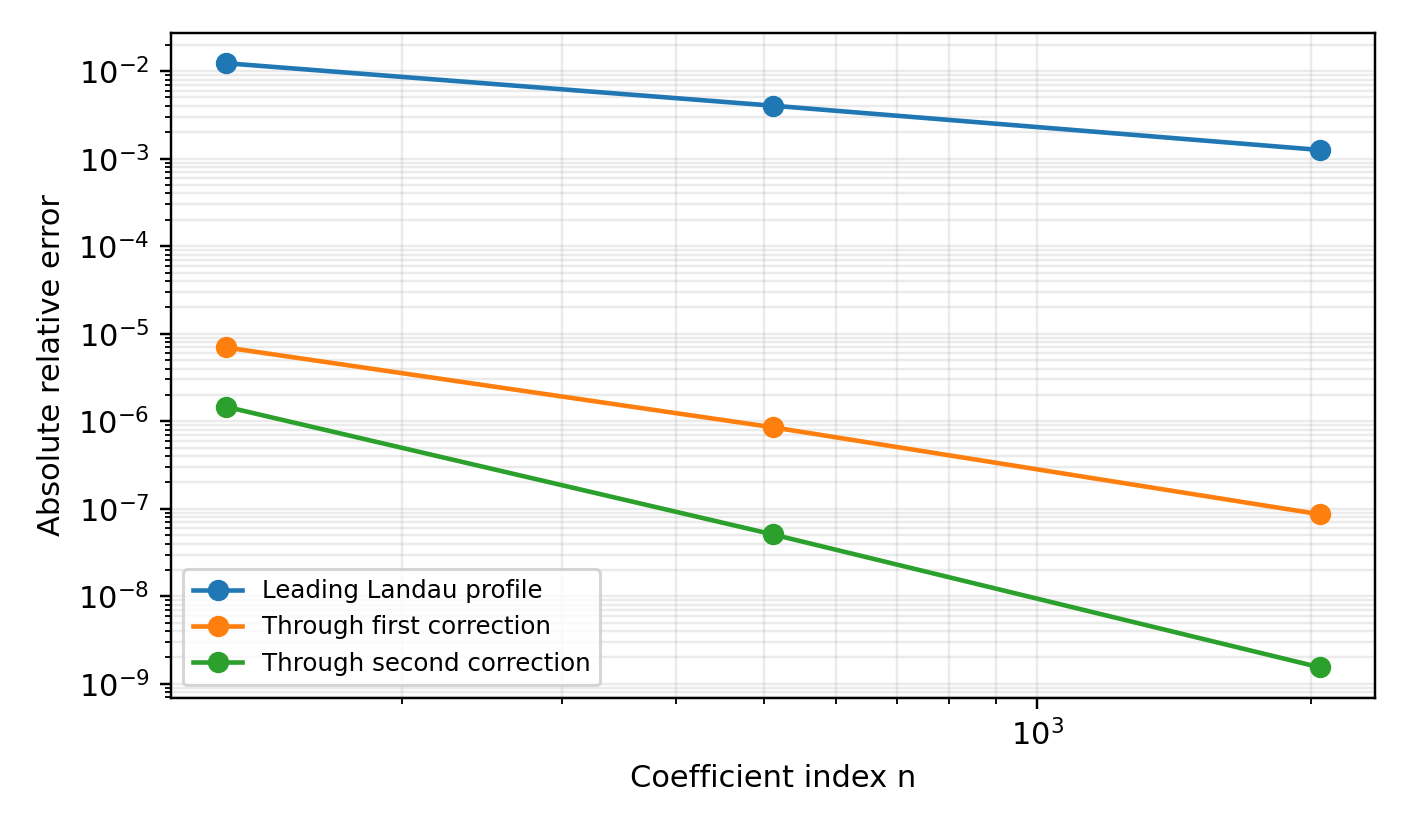
\includegraphics[width=.87\textwidth]{figures/correction_errors.png}
\caption{Absolute relative residuals for \(\la=1\), from the recorded
positive recurrence and independent profile quadrature.}
\label{fig:corrections}
\end{figure}

\subsection{Cutoff profiles and a cancellation-free tail check}
To compute the numerator in \eqref{eq:exact-ratio}, restrict the sum in
\eqref{eq:p-rec} to \(j\le M\) but leave \(p_0\) unchanged. The ratio of
the two target values is then precisely the finite coefficient fraction.
Table~\ref{tab:cutoffs} compares it with \eqref{eq:R-Fourier}, evaluated
at the actual rounded cutoff \(m=M\delta\).
\begin{table}[htbp]
\centering\small
\begin{tabular}{rrrrr}
\toprule
\(\la\)&\(M\)&\(M\delta\)&Finite fraction&Limiting fraction\\
\midrule
1&175&0.5005791&0.4846012&0.4822650\\
1&350&1.0011582&0.9375042&0.9370268\\
1&699&1.9994559&0.9998768&0.9998716\\
4&55&0.5044705&0.0272113&0.0255110\\
4&109&0.9997688&0.5577570&0.5533841\\
4&218&1.9995376&0.9631579&0.9626222\\
\bottomrule
\end{tabular}
\caption{Cutoff diagnostics at \(n=2048\). Convergence need not be rapid
for the smallest cutoffs; no equality of finite and limiting values is claimed.}
\label{tab:cutoffs}
\end{table}

\begin{figure}[htbp]
\centering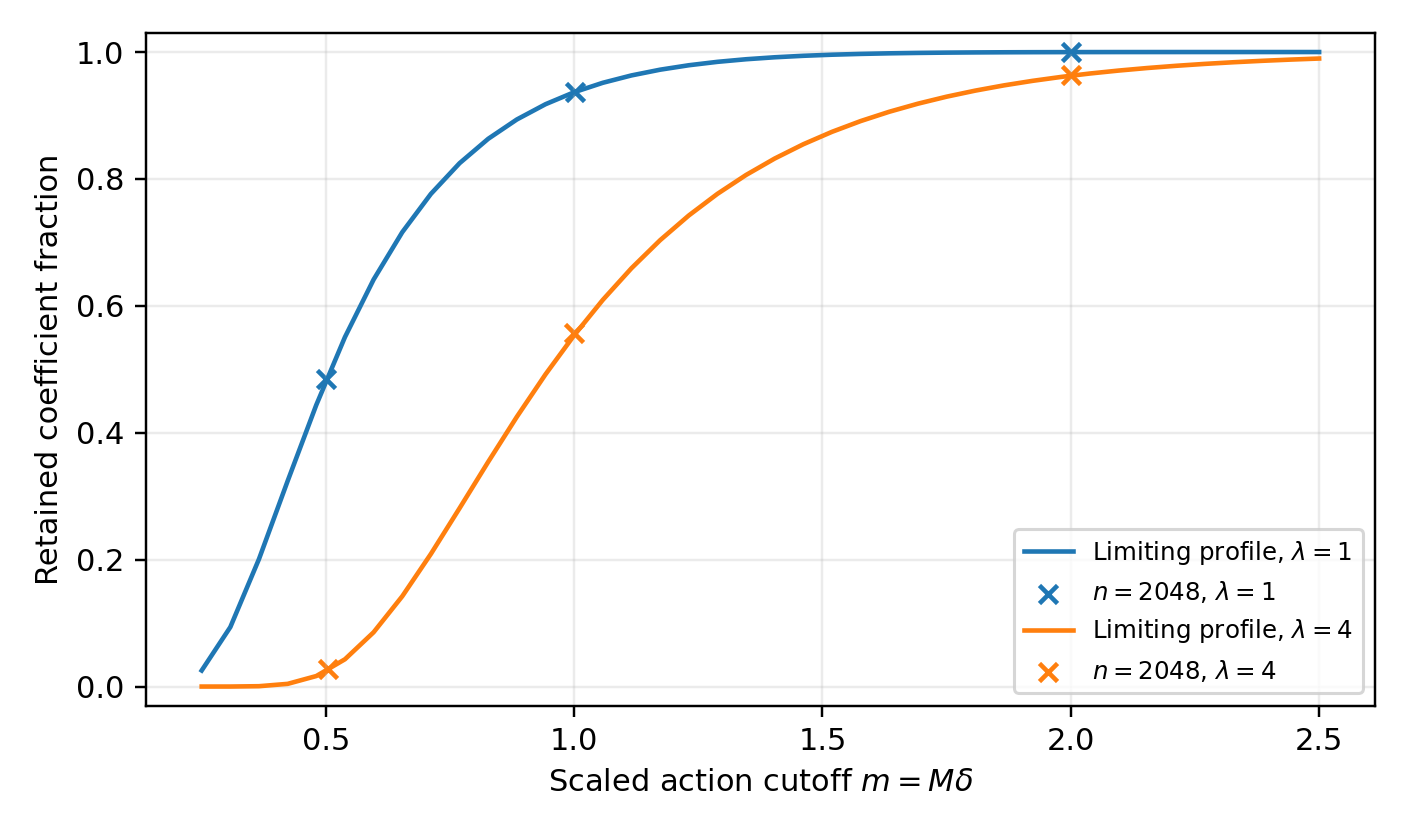
\includegraphics[width=.87\textwidth]{figures/cutoff_profile.png}
\caption{The limiting retention profiles and the independently computed
finite coefficient fractions. All curves are floating-point evaluations
of the formulas in this article.}
\label{fig:cutoffs}
\end{figure}

The program also checks the first Palm moment \eqref{eq:J1-p} against
the proposed equivalent in \eqref{eq:double}, using the rescaled endpoint
variable from the proof. For \(\la=1\), the ratios of the numerically
evaluated \emph{first Palm moment} to that equivalent are
\[
 \begin{array}{c|rrrr}
 m&2&3&4&5\\\hline
 J_1/\text{equivalent}&0.8529573&0.9496008&0.9830888&0.9942918.
 \end{array}
\]
This does not directly numerically measure \(1-\RR\) at extremely small
loss. The passage from \(J_1\) to that loss is proved by the factorial
moment bound in Theorem~\ref{thm:double}. The numerical tail integral
uses a finite upper endpoint in its rescaled variable; its truncation is
not an interval-certified error estimate.

For the independent saddle check,
\(\ee^\la\sqrt{2\pi\la}\HH(\la)\) is integrated in a Gaussian-scaled
variable. The values of
\(\la(\ee^\la\sqrt{2\pi\la}\HH(\la)-1)\) at
\(\la=10,50,100\) are approximately
\(0.0398933,0.0412777,0.0414697\), consistent with the limit
\(1/24\approx0.0416667\). The verification record includes all inputs,
not only these selected rows. Values of a cutoff profile printed as
\(1.0\) can mean numerical saturation; for finite \(m\) the mathematical
profile remains strictly less than one.

\section{Further research questions and concrete next steps}
\label{sec:future}
The following problems are not represented as solved by the results
above. Each has a distinct mathematical target, rather than being a
request to repeat the same calculation with renamed parameters.

\subsection{The boundary-critical side of the lower endpoint}
Our exact normalization assumes an interior fold. For \(\ep>0\), the
paths \(c=1/\zeta(1+\ep)\) and \(c<1/\zeta(1+\ep)\) lie outside it.
Construct a uniform coefficient theorem that includes those paths and
matches the present \(\delta>0\) chart. A natural starting point is the
uncombined expression for \(Q(x)-Q(0)\), retaining both the coupling
mismatch and the nonanalytic power. The main difficulty is to find
coordinates that remain informative when the exact positive saddle
ceases to exist. This is the principal part of the repository's
lower-endpoint problem still left open here.

\subsection{Growing cutoffs and finite-index tolerance certificates}
Prove an error estimate for \eqref{eq:cutoff-limit} that is uniform for
\(m=M\delta\to\infty\). To turn \eqref{eq:tolerance} into a useful
finite-index certificate, the error must be small relative to
\(\exp\{-\la\ee^{m/\la}\}\), not merely \(o(1)\).
A promising route is to apply density-level insertion already in the
finite Poisson model and compare the resulting negative-deviation
local probabilities with their Landau counterparts. This avoids
subtracting two nearly equal coefficient integrals. The relevant
question is the largest joint range of \(m\), \(\delta\), and the target
loss for which the prefactor in \eqref{eq:double} remains valid.

\subsection{An all-orders conditional tail transseries}
The proof of Theorem~\ref{thm:double} can be continued by expanding both
the Landau left tail and the endpoint substitution. Determine a closed
recurrence for the coefficients multiplying
\(\exp\{-\la\ee^{m/\la}\}\), including powers of \(\ee^{-m/\la}\) and
\(1/m\). The multi-jump terms live at much smaller scales involving
\(\exp\{-\la\ee^{km/\la}\}\). A complete hierarchy should state exactly
how these scales interleave and should retain signs in the conversion
from factorial moments to a probability.

\subsection{Simultaneous small-\texorpdfstring{\(\la\)}{lambda} matching}
The small-\(\la\) formula \eqref{eq:Hsmall} is a profile asymptotic.
Develop a finite-coefficient theorem when \(\la\to0\) simultaneously
with \(\delta\to0\), and identify its overlap with a single-large-action
or condensation regime. The Fourier domination used in
Theorem~\ref{thm:crossover} loses strength as \(\la\downarrow0\), so a
new global localization argument is needed. The right-tail logarithm
\(-1-\log\la\) suggests the correct centering, but does not by itself
prove the joint limit.

\subsection{Finite-prefix and slowly varying tail perturbations}
Replace \(j^{-2-\ep}\) by \(j^{-2-\ep}L(j)\), or add a finite
polynomial to the polylogarithm. Determine which perturbations can be
absorbed into the exact saddle, the amplitude \(A\), and finitely many
normal-form coefficients. For a finite prefix the singular part remains
explicit; for a slowly varying \(L\), the effective exponential scale
can change. A useful target is a necessary-and-sufficient hypothesis
under which the same Landau cutoff profile survives after normalization.
No universality assertion for these modified models is made here.

\subsection{The full hierarchy of Gaussian matching obstructions}
Corollary~\ref{cor:matching} isolates the first threshold
\(\la\delta\asymp1\). Subsequent thresholds involve the terms in
\(\la F_{0,\delta}(1)\), such as \(\la\delta^2\).
Develop a minimal renormalization theorem: for a specified joint range,
which finite subset of fold-value terms must be retained to obtain a
relative \(1+o(1)\) approximation? The exact convergent fold-value series
provides the data; the new work is to combine it with an optimally
uniform saddle remainder and to establish necessity as well as
sufficiency of each retained scale.

\subsection{Complex continuation and Stokes geometry}
The inverse charts in Section~\ref{sec:inverse} are local and their
branches are fixed. Continue them around the logarithmic cut and
identify the monodromy of the Landau contour representation.
The fact that a Lambert function occurs in the leading inverse does
not automatically identify all Stokes multipliers of the original
countable-action problem. A satisfactory result should specify the
complex parameter sectors, the admissible contour deformations, and
which exponentially small differences correspond to distinct analytic
solutions rather than to a change of normalization.

\subsection{Arithmetic support and periodic action families}
The full positive support, including action one, supplies the far-arc
attenuation in Lemma~\ref{lem:lattice}. Determine the exact changes for
supports of span greater than one, or for sparse regularly varying
supports. In the periodic case a lattice factor and congruence
restriction should replace the one-saddle formula. In genuinely sparse
cases additional Fourier peaks may survive. An appropriate theorem
should state an arithmetic condition on the support instead of silently
reusing the aperiodic bound.

\subsection{Validated computation at doubly exponential accuracy}
Design a numerical evaluator for \(\log(1-\RR(\la,m))\) with a rigorous
absolute error bound, combining the positive Palm integral with a
certified upper bound for the second factorial moment.
The rescaled integral in the proof of Theorem~\ref{thm:double} removes
both underflow and severe concentration. Interval bounds for its tails
would provide the missing validation layer. This is more useful than
increasing the precision of a subtraction \(1-\RR\) whose conditioning
is already exponentially unfavorable.

\subsection{A staged formalization rather than an unproved interface}
An attainable first stage is a finite polynomial development of
\eqref{eq:Prec}, the exact Lagrange identity in a formal power-series
ring, and the first normal-form coefficients. A second stage can
formalize the scalar analytic implicit chart and its two-sheet
factorization. The uniform local-limit and Palm-tail theorems require
substantial additional measure-theoretic and Fourier infrastructure.
The repository's existing asymptotic-scale modules are relevant
interfaces, but they are not a proof of these new analytical statements.
A useful formalization should keep explicit the distinction between
finite algebraic certificates and quantified asymptotic estimates.

\section{Proof audit, provenance, and reproducibility}
\label{sec:audit}

\subsection{Logical dependencies and remaining boundaries}
The main analytic input is the convergent polylogarithm continuation
formula. The normal-form theorem is an exact algebraic cancellation
applied to that formula. The coefficient theorem then requires three
additional ingredients, all proved here: attenuation on all Fourier
arcs, domination of the growing-contour remainder, and positivity of
the limiting density. Its all-orders endpoint version uses a Taylor
remainder under the same domination, not a purely formal interchange.

The inverse charts use the analytic implicit function theorem and
Cauchy estimates. The Gaussian regime has a separate local-limit proof;
its uniformity is not borrowed from the compact-window theorem.
The cutoff theorem uses a killed characteristic function with the full
centering retained. The sharp loss theorem uses a positive first Palm
integral and a smaller second factorial moment, so its prefactor is not
inferred from an unconditioned tail or from a numerical fit.

All statements labeled theorems, propositions, lemmas, or corollaries in
this article have conventional proofs. There is no claimed resolution
of unrestricted transseries realization, general resurgence, or every
path through the lower critical endpoint. No theorem in this package
has been checked by Lean. Numerical assertions concern only the finite
calculations explicitly recorded. An independent mathematical review
is still needed before treating the draft as refereed research.

\subsection{Repository snapshot and inspection scope}
The inspected repository was \texttt{VladimirReshetnikov/ProveIt}, at
commit
\begin{center}\small\texttt{9250bbf8af80dacf7b252d9d0320b122c80961ba}.\end{center}
This is a commit identifier, not a claim that a mutable branch will
always contain the same content. The connected GitHub tools were used
to inspect the transseries directory tree, its project README, the
series-and-transseries index, and selected package READMEs. The
critical-Hahn package README was read in full. The beginning of its
TeX article, including the exact parametrization, Lagrange coefficient,
and conditional-Poisson formulas, was retrieved; the connector output
for that long source was truncated. We do not claim a complete
line-by-line audit of that article, the large canonical volume, or the
whole repository. The recorded lower-endpoint question is explicit in
the fully retrieved package README.

The recent inverse-digamma, Hahn--Fuchsian, finite-core, signed-quadratic,
and non-Archimedean reversion package summaries were also inspected to
avoid simply repeating an already filed direction. Their mathematical
claims are not assumptions of any theorem here. The source file and
README provenance is listed in the accompanying
\texttt{notes/provenance.json}. No repository file, branch, issue,
or pull request was modified.

\subsection{Classical attribution and novelty status}
The classical parts have been named explicitly: Lagrange inversion,
the simply generated tree/conditioned-allocation connection, the
polylogarithm expansion, the Landau law, the analytic implicit function
theorem, saddle integration, and Poisson insertion. The proposed
research contribution is their proved, explicit combination in the
lower-endpoint model, particularly the confluent normalization,
the matching obstruction, and the conditional cutoff equivalent.
A targeted literature check was made, but it was not an exhaustive
priority search. The present article does not certify that each
formulation appears for the first time in the worldwide literature.

\subsection{Rebuilding and rerunning}
The package contains the LaTeX source \texttt{article.tex}, its
compiled PDF, the figures and recorded data, the verification program,
and a build script. The bibliography is embedded. From the package
root, run
\begin{verbatim}
python -m pip install -r requirements.txt
python verify.py --output build/verification --max-n 2048
sh build.sh
\end{verbatim}
The verification command does not overwrite the recorded \texttt{data/}
outputs. The optional \texttt{make\_figures.py} script regenerates the
figures and its sampled profile data, and therefore does overwrite
those files. Numerical outputs can differ in their final digits across
platforms. On a platform whose \texttt{longdouble} has insufficient
exponent range, the recurrence program raises an explicit error rather
than silently returning an underflowed probability.

The theorem proofs do not require the Python dependencies. The PDF can
be rebuilt from the stored figures with a standard mathematical LaTeX
installation. The accompanying build report records the actual
compilation checks, page count, rendered-page inspection, and file
hashes for this delivered version.

\section{Conclusion}
The lower endpoint is singular in the coupling but regular after exact
fold normalization. At \(\alpha=1\), the fold distance is
\(\delta\sim\ee^{-1/c}\), the sector crossover variable is
\(nc\delta\), and the normalized coefficients are governed by an
explicit Landau profile. The same normalized phase has a convergent
Lambert inverse chart and a uniform square-root chart at its moving
critical value. The first failure of uncorrected Gaussian matching is
quantified by \(\exp(\la\delta/4)\).

Conditioning on the target coefficient has an even stronger effect on
action truncation. The correct limiting budget is \(M\delta\), and
the loss at large scaled cutoff is
\[
 \frac{\sqrt{\la/(2\pi)}}{\HH(\la)m^2}
 \exp\{-m/(2\la)-\la\ee^{m/\la}\}.
\]
The prefactor and the double exponential follow from a positive Palm
integral and a negligible multi-jump correction. These results provide
a concrete interior-fold resolution at the repository's lower
critical endpoint while making the remaining boundary-critical,
finite-tolerance, and complex-continuation questions explicit.

\clearpage
\begin{thebibliography}{9}
\bibitem{repo-critical}
VladimirReshetnikov/ProveIt,
\emph{Beyond Finite-Action Folds: Critical Hahn Transseries, Stable Sector
Asymptotics, and Sharp Action Budgets}, package README and the beginning
of \texttt{article.tex}, including the exact-coordinate propositions.
Research package and editorial amendments, 29 September 2026.
Pinned commit \texttt{9250bbf8af80dacf7b252d9d0320b122c80961ba}.
\url{https://github.com/VladimirReshetnikov/ProveIt/tree/9250bbf8af80dacf7b252d9d0320b122c80961ba/Analysis/Transseries/docs/series-and-transseries/Critical_Hahn_Transseries_Beyond_Finite_Action_Folds}.

\bibitem{repo-index}
VladimirReshetnikov/ProveIt,
\emph{Analysis/Transseries}, project README and documentation index,
same pinned commit, inspected 29 September 2026.
\url{https://github.com/VladimirReshetnikov/ProveIt/tree/9250bbf8af80dacf7b252d9d0320b122c80961ba/Analysis/Transseries}.

\bibitem{janson}
S. Janson,
\emph{Simply generated trees, conditioned Galton--Watson trees, random
allocations and condensation}, Probability Surveys \textbf{9} (2012),
103--252; arXiv:1112.0510.
\url{https://arxiv.org/abs/1112.0510}.

\bibitem{dlmf-polylog}
NIST Digital Library of Mathematical Functions,
\S25.12, \emph{Polylogarithms}, especially Eq.~25.12.12 and its
parameter restrictions. Inspected 29 September 2026.
\url{https://dlmf.nist.gov/25.12}.

\bibitem{bulyak}
E. Bulyak and N. Shul'ga,
\emph{Landau distribution of ionization losses: history, importance,
extensions}, arXiv:2209.06387v1 (2022).
\url{https://arxiv.org/abs/2209.06387}.
The density normalization used in the present paper is fixed explicitly
by \eqref{eq:landau}.

\bibitem{dlmf-lambert}
NIST Digital Library of Mathematical Functions,
\S4.13, \emph{Lambert \(W\)-function}.
\url{https://dlmf.nist.gov/4.13}.
\end{thebibliography}
\end{document}
